

%------------------------------------------------------------------
% $Id: commspec.tex,v 1.5 2008/02/08 18:35:05 chulwoo Exp $
%------------------------------------------------------------------
%Anj: EPCC: e-mail: a.jackson@epcc.ed.ac.uk
%
% For best results, this latex file should be compiled using pdflatex.
% However it will also compile under normal latex, if you prefer.
%
%------------------------------------------------------------------
\documentclass[12pt]{article}

% importing other useful packages:
\usepackage{times}
\usepackage{fullpage}
\usepackage{graphicx}
\usepackage{longtable}
\usepackage{tabularx}
% color for the pdf links:
\usepackage{color}
\definecolor{darkblue}{rgb}{0.0,0.0,0.5}
% for conditional latex source:
\usepackage{ifthen}
% pdftex specifications, these are only included if we are using pdflatex:
\providecommand{\pdfoutput}{0}
\ifthenelse{\pdfoutput = 0}{
% Not PDF:
\usepackage{html}
\newcommand{\hreff}[2]{\htmladdnormallink{#2}{#1}}
}{
% PDF: hyperref for pdf with full linkages:
\usepackage[
pagebackref,
hyperindex,
hyperfigures,
colorlinks,
linkcolor=darkblue,
citecolor=darkblue,
pagecolor=darkblue,
urlcolor=blue,
%bookmarksopen,
pdfpagemode=None,
%=UseOutlines,
pdfhighlight={/I},
pdftitle={QCDSP parallel comms specification \& MPI implementation.  $Revision: 1.5 $ - $Date: 2008/02/08 18:35:05 $.},
pdfauthor={A.N. Jackson \& S. Booth},
plainpages=false
]{hyperref}
}


% Code style commands:
\newcommand{\cls}[1]{{\bf #1}}            % Classes
\newcommand{\struct}[1]{{\bf #1}}         % Structs
\newcommand{\cde}[1]{{\tt #1}}            % Code fragments

% document style modifications:
\setlength{\parskip}{2.0mm}
\setlength{\parindent}{0mm}

% Questionbox commands:
\newcounter{quescount}
\setcounter{quescount}{0}
\newcommand{\quesbox}[2]{\begin{center}\refstepcounter{quescount}\fbox{\parbox{130mm}{
\label{#1}{\bf Q. \arabic{quescount}:} #2} } \end{center} }


% title information:
\title{QCDSP Communications Specification \& the MPI implementation.}
\author{A.N. Jackson \& S. Booth}
\date{\mbox{\small $$Revision: 1.5 $$  $$Date: 2008/02/08 18:35:05 $$}}

%------------------------------------------------------------------
\begin{document}

\maketitle

\tableofcontents
\newpage

%-------------------------------------------------------------------
\section{QCDSP OS Communications}
On QCDSP, the parallel communication subroutines were defined within
the OS, and this will also be the case for QCDOC.  However, for
development purposes, we need a parallel implementation of the code
that can be run here at EPCC while the QCDOC hardware is being
developed.  To do this, we intend to implement the communications
using MPI (v.1), via the interface defined in \cde{sysfunc_cps.h}.  This
interface appears to offer a greater level of functionality than is
currently required, as only a subset of the available subroutines are
used by the C++ QCDSP code.  For now, only the essential elements of
the interface will be included here, while keeping in mind the
possibility of extending the interface as the need arises.

\subsection{Communications Flags}
\label{col:comm:flags}
There are a number of constants defined in \cde{scu\_enum.h} which
associate unique numbers with various communications parameters.  The
first set of definitions identifies the physical directions in which
communications are to be carried out.

\begin{tabular}{llll}
\cde{{\bf enum SCUDir}} & {\bf Name} & {\bf Value} & {\bf Direction} \\
                        &\cde{SCU\_\-TM} & 0 & $-t$\\
                        &\cde{SCU\_\-TP} & 1 & $+t$\\
                        &\cde{SCU\_\-XM} & 2 & $-x$\\
                        &\cde{SCU\_\-XP} & 3 & $+x$\\
                        &\cde{SCU\_\-YM} & 4 & $-y$\\
                        &\cde{SCU\_\-YP} & 5 & $+y$\\
                        &\cde{SCU\_\-ZM} & 6 & $-z$\\
                        &\cde{SCU\_\-ZP} & 7 & $+z$
\end{tabular}

In the case of QCDSP, this actually mapped the physics directions
onto physical wires.  For QCDOC, this will also map onto a set of
wires using the same numbers (0-7), but the actual physical wire being
used will be decided by the OS, for the purposes of machine
partitioning. The four different axes of the system are labelled in a
similar fashion:

\begin{tabular}{llll}
\cde{{\bf enum SCUAxis}} & {\bf Name} & {\bf Value} & {\bf Direction} \\
                        &\cde{SCU\_\-T} & 0 & $t$-axis\\
                        &\cde{SCU\_\-X} & 1 & $x$-axis\\
                        &\cde{SCU\_\-Y} & 2 & $y$-axis\\
                        &\cde{SCU\_\-Z} & 3 & $z$-axis
\end{tabular}

Finally, the communications are labelled as being either sends or receives using:

\begin{tabular}{llll}
\cde{{\bf enum SCUXR}} & {\bf Name} & {\bf Value} & {\bf Meaning} \\
                        &\cde{SCU\_\-REC}  & 0 & Receive from a given direction. \\
                        &\cde{SCU\_\-SEND} & 8 & Send in a given direction.
\end{tabular}

\subsection{Data structures: The SCUDirArg class}
\label{col:comm:data}
Each instance of the \cde{SCUDirArg} class (defined in
\cde{scu\_dir\_arg.h}) describes the type of data-structure to be
transmitted, whether this data should be sent or received, and also
the direction in which the data is to communicated.  The data types
are either contiguous or block-strided, and are defined using the
following parameters:

%\begin{tabular}{llp{110mm}}
\begin{tabularx}{16cm}{llX}
{\bf Type}  & {\bf Name} & {\bf Description} \\
\cde{void$\ast$}  & \cde{addr}       & Base address of the data-block. \\
\cde{SCUDir}      & \cde{dir}        & Direction of this communication. \\
\cde{SCUXR}       & \cde{xr}         & The send or receive flag.\\
\cde{int}         & \cde{blklen}     & Number of elements in each block of data. \\
\cde{int}         & \cde{numblk}     & Number of blocks.\\
\cde{int}         & \cde{stride}     & Number of elements between the
start of the last element of one block and the first element of the successive block.
\end{tabularx}

If this is unclear, consider this simple example of a strided data set:
\begin{center}
  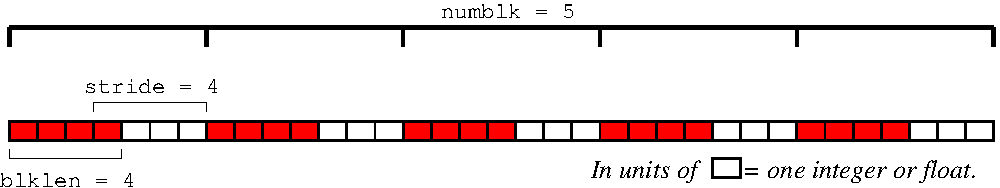
\includegraphics[width=12cm,clip]{stridedef}
\end{center}

The most important issue here, from our perspective, concerns the
units in which both the block-length and the stride are specified.
The unit appears to be the number of \cde{float} or \cde{int}
elements, as opposed to the number of bytes.  This has serious
implications for our aim of allowing both \cde{float} and \cde{double}
precision calculations.  However, if no \cde{int} data is being
transferred between processors, then we can safely assume that the
number of bytes associated with each element is that associated with
the chosen level of precision, and the problem disappears.

A number of methods are also defined by the \cde{SCUDirArg} class to
allow the data-structures to be defined and manipulated.

%----------------------------------
\vspace{5mm}
%\hrule
\cde{SCUDirArg::SCUDirArg (void$\ast$ {\em addr}, {\bf SCUDir} {\em
dir}, {\bf SCUXR} {\em xr}, int {\em blklen}, int {\em numblk} = 1,
int {\em stride} = 1)}

%\hspace{10mm}{}
This constructor allows the parameters
of the communication to be set when an instance of the \cde{SCUDirArg}
class is created.  Note that \cde{numblk} and \cde{stride} will both
default to 1 if other values are not supplied.

%----------------------------------
\vspace{5mm}
%\hrule
\cde{void SCUDir\-Arg::Init (void$\ast$ {\em addr}, {\bf SCUDir} {\em
dir}, {\bf SCUXR} {\em xr}, int {\em blklen}, int {\em numblk} = 1,
int {\em stride} = 1)}

\hspace{10mm}{Used to initialise an `empty' instance of
the SCUDirArg class.  Like the previous constructor subroutine,
\cde{numblk} and \cde{stride} will both default to 1.}

%----------------------------------
\vspace{5mm}
%\hrule
\cde{void$\ast$ SCUDir\-Arg::Addr ()}

\hspace{10mm}{Returns the base address associated with
this \cde{SCUDirArg}.}

%----------------------------------
\vspace{5mm}
%\hrule
\cde{void$\ast$ SCUDir\-Arg::Addr (void$\ast${\em addr})}

%----------------------------------
\vspace{5mm}
%\hrule
\cde{void SCUDir\-Arg::Reload (void$\ast$ {\em a}, int {\em blklen},
int {\em numblk} = 1, int {\em stride} = 1)}

\hspace{10mm}{Used to change the block-length, the number of
blocks and value of the stride.  On QCDSP, this also reloaded the
communication pattern into the DMA.}

%---------------------------------------------------------------
\subsection{The OS Interface}
\label{col:comm:func}
On both QCDSP and QCDOC, the operating system interface is defined in
the header file \cde{sysfunc_cps.h}, apart from standard subroutines such
as \cde{printf} which are defined elsewhere.  In the original
implementation, every subroutine in the communications layer is given
``friend function'' access to the \cde{SCUDirArg} class, so they can
look up the values of the instance variables directly.

%----------------------------------
\vspace{5mm}
%\hrule
\cde{int Unique\-ID ()}

\hspace{10mm}{Returns a number which is unique for each
node.  These numbers have no particular significance, but one part of
the library does attempt to used them to seed an RNG, and therefore
zerois not advisable.}

%----------------------------------
\vspace{5mm}
%\hrule
\cde{int Coor\-T ()}\\
\cde{int Coor\-X ()}\\
\cde{int Coor\-Y ()}\\
\cde{int Coor\-Z ()}

\hspace{10mm}{Functions to return four-dimensional
coordinates of the node.}

%----------------------------------
\vspace{5mm}
%\hrule
\cde{int Size\-T ()}\\
\cde{int Size\-X ()}\\
\cde{int Size\-Y ()}\\
\cde{int Size\-Z ()}

\hspace{10mm}{Functions to return the size of the 4-D processor
grid in each direction.}

%----------------------------------
\vspace{5mm}
%\hrule
\cde{int Num\-Nodes ()}

\hspace{10mm}{Returns the total number of nodes.}

%----------------------------------
\vspace{5mm}
%\hrule
\cde{unsigned int Seed ()}\\
\cde{unsigned int Seed\-S ()}\\
\cde{unsigned int Seed\-T ()}\\
\cde{unsigned int Seed\-ST ()}

\hspace{10mm}{For initialising the random number seeds,
using numbers which on QCDSP were loaded at boot time. For
\cde{Seed()}, the seed is different for each node and is changed every
time the machine is reset. \cde{Seed\-S} is the same for each node
(spatially fixed, hence the S), but changes in time. \cde{Seed\-T} is
different for each node, but is fixed in time (the T), so it is
unchanged by a reset. \cde{Seed\-ST} is the same for each node
(spatially fixed, hence the S), and the same after every reset (fixed
time, hence T).}

%----------------------------------
\vspace{5mm}
%\hrule
\cde{unsigned int sync ()}

\hspace{10mm}{Synchronises all the processors.}

%----------------------------------
\vspace{5mm}
%\hrule
\cde{int SCURemap ({\bf SCUDir} {\em dir})}

\hspace{10mm}{
This subroutine looks up the `wire number' associated with a given
direction.  This can be used to create a mapping table, which maps
directions \#0-7 onto wires \#0-7 in whichever order is most
appropriate.}

%----------------------------------
\vspace{5mm}
%\hrule
\cde{void SCUTrans ({\bf SCUDir\-Arg}$\ast$ {\em arg})}

\hspace{10mm}{
Performs a single data-transfer, as specified by the \cde{SCUDirArg}
object pointed to by \cde{arg}.}

%----------------------------------
\vspace{5mm}
%\hrule
\cde{void SCUTrans ({\bf SCUDir\-Arg}$\ast\ast$ {\em arg}, int {\em n})}

\hspace{10mm}{ Used to perform \cde{n} simultaneous
data-transfers, as specified by the array of \cde{SCUDirArg} objects
passed through \cde{arg}.  }

%----------------------------------
\vspace{5mm}
%\hrule
\cde{void SCUTrans ({\bf SCUDir\-Arg}$\ast$ {\em arg}, unsigned
int$\ast$ {\em offset}, int {\em n})}

\hspace{10mm}{ Perform \cde{n} transfers, all of which
have the same block, stride and number of blocks, but have different
addresses.  Each transfer is started at a specified offset
(\cde{offset[i]}) relative to the base-address held in the
\cde{SCUDirArg}.}

%----------------------------------
\vspace{5mm}
%\hrule
\cde{void SCUSet\-DMA ({\bf SCUDir\-Arg}$\ast$ {\em arg})}\\
\cde{void SCUSet\-DMA ({\bf SCUDir\-Arg}$\ast$$\ast$ {\em arg}, int
{\em n})}

\hspace{10mm}{On QCDSP, this is used to set up the DMA,
using the array of comms definitions held in \cde{arg} (no transfers
are done).}

%----------------------------------
\cde{void SCUTrans\-Addr ({\bf SCUDir\-Arg}$\ast$ {\em arg})}\\
\cde{void SCUTrans\-Addr ({\bf SCUDir\-Arg}$\ast$$\ast$ {\em arg},
int {\em n})}

\hspace{10mm}{This function performs SCU transfers, but
does not alter the existing block, stride and number of blocks held in
the registers of the SCU.  This call must be preceded by a
\cde{SCUSetDMA} call.  The base-addresses of the data to be
communicated are taken from the array \cde{SCUDirArg} objects pointed
to by \cde{arg}. }

%----------------------------------
\vspace{5mm}
%\hrule
\cde{void SCUTrans\-Complete ()}

\hspace{10mm}{The function does not
return until all of the transfers on this PE have been completed.}

\subsection{Questions concerning the interface.}
These last few points can be resolved when we have access
to the original \cde{scu\_dir\_arg.C} from the QCDSP code.
\begin{itemize}
\item \cde{Addr()} is assumed to set the base-address of this instance of
\cde{SCUDirArg} to \cde{addr}, and then returns the \emph{previous}
base-address. Is this the case.
\item Has the \cde{Reload()} command been interpreted correctly?
\end{itemize}

%--------------------------------------------------------------------
\newpage
\section{MPI Implementation: MPI-SCU}
\subsection{Introduction}
The MPI implementation of the QCDSP SCU layer is a stand-alone system,
which may be compiled with or without the QCDSP code.  Only MPI
version 1 directives are used.

\subsection{Contents Of This Distribution}
The MPI-SCU distribution contains the following files:

\begin{tabular}{l|l}
{\bf File} & {\bf Description} \\
\hline
%
\cde{scu\_enum.h} & Slightly modified re-implementation of the
communications enums. \\
\cde{scu\_dir\_arg.h} & Headers for the data-structure definition routines. \\
\cde{scu\_dir\_arg.C} & Implementation of the above. \\
\cde{sysfunc_cps.h} & Headers for the MPI-emulated QOS calls. \\
\cde{sysfunc.C} & Implementation of the above. \\
\cde{mpi\_requests.h} & Source for the MPI-implementation-specific request handler. \\
\cde{Makefile} & Makefile for the MPI-SCU library. Does not make the test-programs. \\
\cde{commsMPI.def} & Example comms-definition file. \\
\cde{doc/} & MPI-SCU documentation, including this file. \\
\cde{lib/} & Directory where the MPI-SCU library is placed. \\
\cde{test/} & Directory for MPI-SCU test programs. \\
%
\end{tabular}

Note that the MPI-SCU Makefile will have to altered in order to work at an
institution other that EPCC.  The parts that will need to be altered
are specified at the top of the Makefile, and concern the MPI compiler
name and include/link paths.

\subsection{Integrating MPI-SCU Into The QCDSP Code}
It should be fairly straightforward to integrate the MPI-SCU library into
the QCDSP code.
\begin{itemize}
\item Compile the MPI-SCU library on its own (see the above point concerning the
Makefile's portability).
\item Add the \cde{.../MPI-SCU/} directory to the include path.
\item Add the \cde{.../MPI-SCU/lib/} directory to the link path.  
\item Add the \cde{-lcommsMPI} flag to the compile/link command.
\end{itemize}
The only problem could be that any given version of the QCDSP code may
contain its own versions of some of the files in this distribution (in
particular, \cde{scu\_enum.h}).  For now, we suggest simply moving the
non-MPI versions of the conflicting files out of the way. In the
future, this should be remedied by adding a suitable MPI flag to the
QCDSP code's Makefile.

\subsection{Compiler Options}
These compiler switches specify some of the basic parameters of the
MPI-SCU layer.  All of these can be overridden in the Makefile, using
the \cde{-D} flag in the compiler flags.

%\begin{tabular}{l|l|p{80mm}}
\begin{tabularx}{16cm}{l|l|X}
{\bf Name} & {\bf Default} & {\bf Description}\\
\hline
\cde{VERBOSE} & \cde{UNDEFINED} & Outputs detailed information
concerning the comms calls to a set of log-files (one for each
processor).\\
\hline
\cde{NDIM} & \cde{4} & Dimensionality of the system.  Currently, only NDIM = 4 is
meaningful because the interface does not allow access to anything
other than 4 dimensions. \\
\hline
\cde{COMMS\_ENVVAR} & \cde{"COMMS\_DEF"} & Name of the environment variable used
to specify the run-time parameters of the MPI-SCU layer.  If no such
environment variable exists, then the \cde{COMMS\_DEFFILE} is
used instead.\\
\hline
\cde{COMMS\_DEFFILE} & \cde{"commsMPI.def"} & Default filename
(relative to the location of the executable) of a file that contains
the run-time parameters of the MPI-SCU layer.  \\
\hline
\cde{COMMS\_DATASIZE} & \cde{4} & Default size (in bytes) of
the fundamental data type to be transferred between processors
(i.e. the size of integer or floating-point numbers). This can be
overridden at the software (\cde{SCUDirArg}) level.\\
\end{tabularx}

\subsection{Run-time Control}
The parallel environment of the code can be specified at run-time, via
the environment variable specified by \cde{COMMS\_ENVVAR}, or the file
specified by \cde{COMMS\_DEFFILE}.  The environment variable can
either directly specify the MPI-SCU parameters, or point to a file
containing those definitions.  The definitions themselves consist of a
series of tag \& value pairs, in the format \cde{\{NAME=}value{\}},
specifying the following aspects of the parallel environment:

%\begin{tabular}{l|l|p{65mm}|l}
\begin{tabularx}{16cm}{l|l|X|l}
{\bf Item} & {\bf Level} & {\bf Description} & {\bf Default} \\ 
\hline
\cde{\{GRID=}t,x,y,z\cde{\}} & REQUIRED & Defines the number of processors in each
direction.  & n/a \\
\hline
\cde{\{LOGFILE=}$\langle$filename$\rangle$\cde{\}} & Optional & This should specify the absolute or
relative path of a file to which \cde{VERBOSE} textual output should be placed.  If its value is \cde{stderr} or \cde{stdout} that stream is used instead. & \cde{comlog} \\
\hline
\cde{\{SEED=}$\langle$integer$\rangle$\cde{\}} & Optional & Specify the RNG seed that SeedS or SeedST will
return & \cde{1} \\
\hline
\cde{\{SEEDFILE=}$\langle$filename$\rangle$\cde{\}} & Optional & Specifies a file containing a 
number of RNG seeds.  This is used by Seed and SeedT to define a
different seed for every processor. & \cde{rng.dat} \\
\end{tabularx}

The environment variable is determined as either pointing to a file or
containing the tags based on the whether or not it contains a ``\{'' or not
(ignoring whitespace).  The contents of the string or the file is
turned into a stream of tokens, using the characters [\{\} ,=$\backslash$n$\backslash$t] as
delimiting whitespace.  The order of the definition items is not
important, but the case is.

For example, consider setting the environment variable to a filename
(in bash)
\begin{verbatim}
export COMMS_DEF="commsMPI.def"
\end{verbatim}
where the file \cde{commsMPI.def} contains the following information:
\begin{verbatim}
{ GRID = 64,32,32,32 }
{ LOGFILE = comms.log }
{ SEED = 128366328 }{ SEEDFILE = rngseeds.dat }
\end{verbatim}
This will use a $(t,x,y,z) = 64{\times}32{\times}32{\times}32$
processor grid, and all \cde{VERBOSE} output will be sent to log-files
called \cde{comms.log.X} where \cde{X} is the processor number.
\cde{SeedS()} \& \cde{SeedST()} will return \cde{128366328}, and
\cde{Seed()} \& \cde{SeedT()} will return a RNG seed taken from the
file \cde{rndseeds.dat}.  

This could also be achieved using the environment variable alone.  For
example, in \cde{bash} one can use:
\begin{verbatim}  
export COMMS_DEF="{LOGFILE=comms.log}{SEED=128366328}
{GRID=64,32,32,32}{SEEDFILE=rngseeds.dat}"
\end{verbatim}
This will produce exactly the same behaviour as the previous
file-based approach.

\subsection{The Communications Flags}
The flags specified by \cde{scu\_enum.h} have only been changed very
slightly:  An extra flag has been added to the end of each enum to
clearly distinguish between undefined and defined values.

Enumeration \cde{SCUDir} now also defines \cde{SCU\_NoDir = -1}.\\
Enumeration \cde{SCUAxis} now also defines \cde{SCU\_NoAxis = -1}.\\
Enumeration \cde{SCUXR} now also defines \cde{SCU\_NoXR = -1}.

\subsection{The SCUDirArg Class}
Each instance of the \cde{SCUDirArg} class defines and commits a
MPI\_Datatype appropriate for the specified number of blocks,
block-length and stride.  The basic data type is always defined as
being floating-point, but the number of bytes for each float (which
defaults to \cde{COMMS\_DATASIZE}) an be specified using the following
method:\\
\cde{SCUDirArg::SetDataSize( int mpi\_datasize);}\\
where the integer argument specifies the number of bytes required for
every element of data.  For example, if we wish to use an instance of
\cde{SCUDirArg} called \cde{scudat} to transfer \cde{double} data, we
simply set:\\
\cde{scudat.SetDataSize(8)}

This class also defines a few extra methods to allow the OS interface
to access the MPI datatype and other data-transfer parameters.  These
are straightforward, and are described in the \cde{scu\_dir\_arg.h}
header file.

\subsection{The OS Interface}
The subroutines defined in \S\ref{col:comm:func} have all been
implemented in this version of MPI-SCU.  As well as these, the MPI
version adds a number of new interface routines:

\cde{void SCUCommsInit( void );}

\hspace{10mm}{Initialisation: Parses the communication parameters, calls
\cde{MPI\_Init}, etc.  This will be called automatically when the code
attempts to perform any \cde{SCUDirArg} operations, but is supplied here so that
it can be explicitly called at the start of the program.}

\cde{void SCUGlobalSum(Type\_tag t, size\_t tsize, int n, void $\ast$ivec, void $\ast$ovec );}

\hspace{10mm}{Perform a global sum directly using
\cde{MPI\_Allreduce}.  This avoids using the standard global sum
calculation, which is implemented via a set of \cde{SCUTrans} calls,
and so this version will probably be more efficient on most
architectures.  The results are sent to all processors.\\
\cde{Type\_tag t} Indicates the type of the data: one of \cde{TYPE\_float} \& \cde{TYPE\_int}.\\
\cde{size\_t tsize} Indicates the size of the individual
floats or ints (in bytes).\\
\cde{int n} The number of items to be summed.\\
\cde{void $\ast$ivec} The input vector for the summation.\\
\cde{void $\ast$ovec} The output vector for the summed result.\\
}

\cde{void SCURaiseError( char$\ast$ errstr );}\\
\cde{void SCURaiseError( const char$\ast$ errstring );}

\hspace{10mm}{Wrapper for the comms-error reporting
mechanism.  This currently prints the error to the standard output and
then exits, but will eventually be made to use the QCDSP code's error
reporting mechanism (the \cde{Error} class).}

Note that the implementation only identifies data transfers by their
direction, but that MPI retains the order of communications.
Therefore, multiple transfers in a single direction will work as long
as the order of the send commands matches the order of the receives.

\subsection{Test Programs}
There is currently a single test program for the MPI-SCU layer, which
also does not require the QCDSP code in order to work.  The next stage
will be add a test based on the original SCU-based global sum which
will also compare this mechanism to the \cde{SCUGlobalSum} routine.
In the longer term, the aim will be to get one of the dynamical Wilson
fermion test-codes running via MPI-SCU.

\subsubsection{\cde{tests/simple/commstest.C}}
This tests the parsing of the communication parameters, and sets up a
few strided and contiguous \cde{float}, \cde{int} and \cde{double}
transfers between processors.  The data thus transmitted is checked
for correctness at every stage.  See the source files for more
information.

\subsubsection{\cde{tests/stride/stridetest.C}}
To test that the stride had been correctly implemented in MPI, this
code (from GF) was compiled and tested on QCDSP, and then re-compiled
and re-tested using the MPI-SCU layer here at EPCC.  The results were
identical.  The original QCDSP code did not call SCUTransComplete, and
in the MPI version this lead to incorrect answers.  On QCDSP, it may
be possible to skip the SCUTransComplete call under certain
conditions, but this cannot be supported in the MPI implementation.

\subsection{Unresolved Issues}
\begin{itemize}
\item The entire \cde{sysfunc} interface cannot be made \cde{extern
"C"}, because there are overloaded subroutines.  If external code
requires access to the communication-calls with un-munged names, some
kind of wrapping or selective \cde{extern "C"} usage may be required.

\item In QCDSP, only the root processor could actually perform input
and output, whereas under MPI all processors can write to disk.
Therefore, as things stand, the code will produce multiple identical
output files.  This may cause more serious problems for
the \emph{inputting} of data files.

\item On a related point, in its current formulation, the MPI-SCU
layer works be allowing \emph{all} processors to access the various
definitions files.  This is simpler than only allowing a single
processor to read the files and then distributing the data, but may
cause problems on some platforms.

\item The request handler defined in \cde{mpi\_requests.h} is
currently rather poor, and has an arbitrary upper limit of 100
requests per node.  This will be changed to handle things properly,
via a linked list.
\end{itemize}

\end{document}









